\documentclass[10pt,letterpaper]{article}
\usepackage[top=0.85in,left=1.00in,footskip=0.75in]{geometry}
% Use Unicode characters when possible
\usepackage[utf8]{inputenc}
% amsmath and amssymb packages, useful for mathematical formulas and symbols
\usepackage{amsmath,amssymb}
% cite package, to clean up citations in the main text. Do not remove.
\usepackage{cite}
%\usepackage[round]{natbib}

% Use nameref to cite supporting information files (see Supporting Information section for more info)
\usepackage{nameref,hyperref}

% ligatures disabled
\usepackage{microtype}
\DisableLigatures[f]{encoding = *, family = *}

% rotating package for sideways tables
\usepackage{rotating}

% Remove comment for double spacing
%\usepackage{setspace}
%\doublespacing

%\textwidth 5.25in
\textheight 8.75in

% Bold the 'Figure #' in the caption and separate it from the title/caption with a period
% Captions will be left justified
\usepackage[aboveskip=1pt,labelfont=bf,labelsep=period,justification=raggedright,singlelinecheck=off]{caption}

% Use the PLoS provided BiBTeX style
%\bibliographystyle{plos2009}

% Remove brackets from numbering in List of References
\makeatletter
\renewcommand{\@biblabel}[1]{\quad#1.}
\makeatother
%%%%%%%%%%%%%%%%%%%%%%%%%%%%%%%%%%%%%%%%%%%%%%%%%%%%%%%%
%%%%%%%%%%%% OPTIONAL MACRO DEFINITIONS %%%%%%%%%%%%%%%%
%%%%%%%%%%%%%%%%%%%%%%%%%%%%%%%%%%%%%%%%%%%%%%%%%%%%%%%%

\newcommand\globalScalePlots{1}

% For commenting
\usepackage{color} % ULTIMATELY delete since I can't have colored text???
\usepackage[normalem]{ulem} % For strike-out text during editing

\usepackage[dvipsnames]{xcolor}
\newcommand{\nathanComment}[1]{\textcolor{Emerald}{(NB:~#1)}}
\newcommand{\stephanieComment}[1]{\textcolor{BrickRed}{(SB:~#1)}}
\newcommand{\robComment}[1]{\textcolor{Orange}{(RP:~#1)}}

% To define more useful LaTeX commands
\usepackage{xparse}

% Equation referencing
\DeclareDocumentCommand \eref{oooo} {\IfNoValueTF{#2}{Eq.~(\ref{#1})}{\IfNoValueTF{#3}{Eqs.~(\ref{#1}) and (\ref{#2})}{\IfNoValueTF{#4}{Eqs.~(\ref{#1})-(\ref{#3})}{Eqs.~(\ref{#1})-(\ref{#4})}}}}

\newcommand{\bareEq}[1]{(\ref{#1})} % Equations

% Figure referencing
\DeclareDocumentCommand \fref{ooo} {\IfNoValueTF{#2}{Fig.~\ref{#1}}{\IfNoValueTF{#3}{Figs.~\ref{#1} and \ref{#2}}{Figs.~\ref{#1}-\ref{#3}}}}

% Letters for figure sub-parts
\newcommand{\letter}[1]{#1} % For main text. Ex: As shown in Fig. 12A
\newcommand{\letterParen}[1]{(#1)} % For captions. Ex: (A) Low limit and (B) high limit

% Shortcuts for often-used symbols that may change notation
\newcommand{\K}{K_{\text{DNA}}}
\newcommand \foldchange{\operatorname{fold-change}}
\newcommand{\Rtot}{R_{\text{Tot}}}
\newcommand{\KIeff}{\tilde{K}_I} % Effective KI constant

%% END MACROS SECTION


\begin{document}

\title{Remaining experiments for Onew}
\maketitle

We experienced some delays this summer for finishing Onew. However, the number of remaining experiments required to finish the paper is modest and they can be completed on the 1-2 month timescale. There are a number of additional experiments which, while not essential, may strengthen the paper. In this writeup I discuss the status of the experiments required to finish the paper (in the section ``Essential experiments'') and discuss potential additional experiments and their timelines (``Additional Experiments'').

\section*{Essential experiments}

We have a small number of experiments that still need to be completed before the
minimal version of the paper can be finished. Specifically, we need to finish
collecting flow cytometry data for repressor titrations of the 3+ bp mutants,
we need to finish collecting flow cytometry data for IPTG titrations of the 1 bp
mutants, and we need a few Sort-Seq replicates so that we can quantify the
amount of variation inherent in producing an energy matrix.

\subsection*{3+ bp mutants}
One of the aims of this study is to determine how well our Sort-Seq energy
matrices predict the binding energies of operator mutants. We already have data
for 1 bp and 2 bp mutants ($\sim$ 10 of each type of mutant, see Fig
\ref{fig:pred_v_fit}). We wish to extend this data set to include $\sim$ 10 3
bp mutants and several 4+ bp mutants so that we may refine our analysis of how
the quality of the predictions deteriorates as the number of mutations grows
larger.\\

\begin{figure}[ht!]
\begin{center}
\scalebox{0.6}{\includegraphics{graphics/pred_vs_measured_box}}
\caption{\textbf{Energy matrix predictions are accurate for small sequence
deviations.} Binding energies $\Delta \varepsilon_R$ for each mutant operator
were obtained using two methods. First, $\Delta \varepsilon_R$ was measured by
fitting to fold-change data. Then, $\Delta \varepsilon_R$ was predicted using
an energy matrix. (A) Measured values for $\Delta \varepsilon_R$ are plotted
against the corresponding predicted values. If predictions are perfectly
accurate, they will fall along the gray dotted line. Predictions for single
base pair mutants (circles) and two base pair mutants (squares) are generally
accurate, although the single base pair predictions are superior to the two
base pair predictions. (B) Prediction accuracies for multiple base pair mutants
were measured by generating predictions from matrices based on O2 and O3, each
of which differs by several base pairs from the mutant operators whose binding
energies were measured. On average, predictions are accurate to within $\sim 1\
k_BT$ for up to $m = 4$, but for $m \geq 5$ the accuracy falls off
considerably. }
\label{fig:pred_v_fit}
\end{center}
\end{figure}

\noindent \textbf{Status:} A set of eight 3 bp mutants, each with the full range of
repressor copy numbers, has been made and checked via sequencing. These are
ready for measurement by flow cytometry. A set of five 4+ bp mutants with the
full range of repressor copy numbers is currently being made.\\

\noindent \textbf{Timeline:} Barring any technical difficulties, data
acquisition for the 3 bp mutants should be completed by Sep 29. Strain
construction for the 4+ bp mutants will be completed by then as well. Data
acquisition for the 4+ bp mutants should be completed by Oct 14.

\subsection*{IPTG titrations}

The purpose of the ITPG titration experiments is to show that Sort-Seq derived
energy matrices, in conjunction with a quantitative model like MWC, make it
possible to design specific induction responses. Figure
\ref{fig:designed_induction} shows the data we have so far for designed
induction responses. The data shown here represent only a few replicates, so to
finish data acqusition we will need to a) take a few more replicates with the
strains shown here and b) acquire data for the remaining 1 bp mutants to
demonstrate the consistency of our induction predictions.\\

\begin{figure}[ht!]
\begin{center}
\scalebox{0.6}{\includegraphics{graphics/designed_phenotype}}
\caption{\textbf{Energy matrix predictions can be used to design precise
phenotypic responses} (A) Phenotypic parameters (leakiness, saturation, and dynamic
range) exhibit trade-offs as $\Delta \varepsilon_R$ is varied. Maximizing
saturation or minimizing leakiness can only be achieved by reducing the dynamic
range below its maximum. (B) Operators with different values of $\Delta
\varepsilon_R$ were chosen to have varying induction responses based on the
phenotypic trade-offs shown in Part A. The induction responses predicted based
on energy matrix predictions (dashed lines) generally agree well with the
responses predicted based on measured $\Delta \varepsilon_R$ values for each
operator. The data likewise indicate that specific induction phenotypes can be
designed by making operator mutations as informed by energy matrix predictions.}
\label{fig:designed_induction}
\end{center}
\end{figure}

\noindent \textbf{Status:} 2-3 replicates have been taken for each of the
operators shown in Fig \ref{fig:designed_induction}. Data acquisition has not
started for the remaining 1 bp operators.\\

\noindent \textbf{Timeline:} Barring any technical difficulties, all data could
be acquired by Nov 3.

\subsection*{Sort-Seq replicates}

In an effort to obtain the highest-quality Sort-Seq data possible, we performed
Sort-Seq in multiple genetic backgrounds in which the repressor copy number was
varied. We expected that increasing the number of repressors present in the cell
would amplify the effects of mutations to the operator and thus give us more
accurate data. Figure \ref{fig:seq_logos} shows how the sequence logos for each
operator vary with repressor copy number. O2 appears to be particularly
sensitive to repressor copy number, with the logo's total information
increasing noticeably as the repressor copy number is increased. In order to
determine whether this is a real effect, however, we need to perform multiple
Sort-Seq replicates in the same genetic background in order to establish the
amount of variation that can be observed from experiment to experiment. I plan
on performing two additional Sort-Seq replicates each for O1 RBS1147,
O1 RBS446, O2 RBS1147, and O2 RBS446.  \\

\begin{figure}[ht!]
\begin{center}
\scalebox{0.6}{\includegraphics{graphics/all_seq_logos}}
\caption{\textbf{Sequence logos acquired from Sort-Seq in different genetic backgrounds.} Sort-Seq was performed for O1, O2, and O3 in strains with repressor tetramer copy number $R = 30$, 62, 130, or 610. While the effect of repressor copy number on O1 and O3 appears to be minimal, it appears that increasing the repressor copy number measurably increases the information content of the logos generated for O2.  }
\label{fig:seq_logos}
\end{center}
\end{figure}

\noindent \textbf{Status:} Not started.\\

\noindent \textbf{Timeline:} Replicates can be sorted and sent for sequencing by Oct 6.
Sequence analysis can be performed within a week after receiving the sequences.

\section*{Additional experiments}

The suggested additional experiments are discussed below and ranked in order of priority.

\subsection*{Priority 1: regulatory context}

As discussed in Alaska, I have been considering extending the study to include
comparisons of the energy matrices we get when operators are placed in different
regulatory contexts. Several people voiced an interest in this idea in Alaska,
and I think it would be a good way to both address potential limitations of our
method and potentially include some new scientific insights so that this is not
solely a methods paper. My idea is that we would use our knowledge of
\textit{lac} repression to design several constructs that we expect to cause
repression using different mechanisms. As shown schematically in Fig
\ref{fig:reg_contexts}, this would include simple repression with an operator
positioned at +20 or -50 \cite{Garcia2012} or repression by looping
\cite{Boedicker2013}. We would compare Sort-Seq derived energy matrices and/or
sequence logos for each of these operator locations to assess the extent to
which binding affinities change as regulatory context changes. We can also use
data from Nathan's paper to explore this question. For example, the two XylR
binding sites he identifies provide an example of sites whose sequence
preferences change based on context, while moving PurR from approximately -20
to +10 does not appear to alter the sequence preference.\\

\begin{figure}[ht!]
\begin{center}
\scalebox{0.6}{\includegraphics{graphics/onew_reg_contexts}}
\caption{\textbf{Alternative regulatory contexts for \textit{lac} repressor.} These schematics show four different regulatory contextsw for \textit{lac} repressor that have already been studied by our lab in some capacity. Performing Sort-Seq in each of these contexts, with separate Sort-Seq experiments for the main (downstream) and auxiliary (upstream) looping operators, would allow us to compare how sequence preferences are altered by changes in regulatory context that change the mechanism of regulation.}
\label{fig:reg_contexts}
\end{center}
\end{figure}

\noindent \textbf{Status:} Oligos for these constructs have already been designed and I
have received them from IDT. Wild-type constructs for each promoter have been
made on plasmid and confirmed via sequencing. Library plasmids are partially completed for the operator at -50 and an auxiliary looping operator. Some debugging needs to be done for the library plasmids of the operator at +20 and the main looping operator.\\

\noindent \textbf{Timeline:} If we wish to proceed only with the constructs that aren't giving us trouble (i.e. operator at -50 and auxiliary looping operator), strain construction can be finished by Sep 29 and sorting can be completed by Oct 14. Sequence analysis can be finished
within a week after sequencing results return.\\

\noindent Otherwise, if we wish to proceed with all of the constructs (which would include the operator at +20 and the main looping operator), strain construction would most likely not be finished until the beginning of November. Sorting could then be completed by mid-November.

\subsection*{Priority 2: low-affinity binding sites}

A finding from previous studies is that it is difficult to predict the
binding energies of low-affinity binding sites \cite{Zuo2014, Maerkl2007, Siebert2016}. Figure \ref{fig:low_affinity} shows predicted vs measured binding
affinities from Ref. \cite{Siebert2016}(presented as the log ratio of dissociation constants, $\log{\frac{K_d}{K_{d, ref}}}$). They find that while predicting the binding energies of 1 bp mutants from a linear PWM produces satisfactory results (blue), predicting the binding energies for low-affinity mutants with multiple mutations is unsuccessful (orange). \\

\noindent We find similar results; if we try to predict the binding energies of sequences with several mutations, our predictions become quite poor. However, I think that this is not necessarily due to the low-affinity nature of these sites, but rather the degree of distance from the sequence used to create the energy matrix. I think it would be interesting to test this idea by making a series of low affinity mutants that have 1 bp mutations relative to O3 (rather than O1, which has been our standard). Then, we can assess whether the O3 energy matrix accurately predicts the binding affinities of these mutants, and compare these predictions to predictions from the O1 energy matrix. \\

\begin{figure}[ht!]
\begin{center}
\scalebox{0.75}{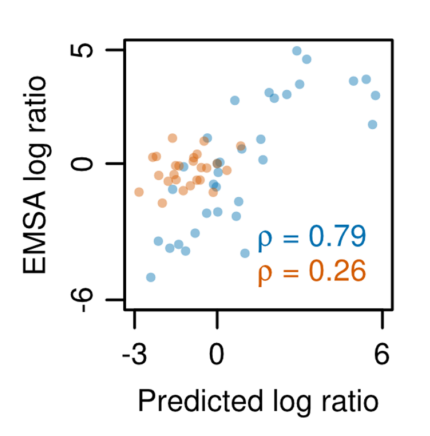
\includegraphics{graphics/low_affinity}}
\caption{\textbf{Failure to predict low-affinity binding sites.} Data from Ref \cite{Siebert2016} showing PWM predictions versus measurements from electrophoretic mobility shift assays (EMSAs) for single base-pair mutants (blue) and low-affinity mutants with multiple mutations (orange). They find that while the PWMs perform well for the single base pair mutants, they perform poorly for the low-affinity mutants.}
\label{fig:low_affinity}
\end{center}
\end{figure}

\noindent \textbf{Status:} Not started.

\noindent \textbf{Timeline:} My experiment calendar is full through the end of October. So, the new O3-based constructs could be made in November and the flow experiments could be completed in December.


\subsection*{Priority 3: ``averaged'' versus ``strict'' linear model}

Multiple studies \cite{Zuo2014, Maerkl2007} have shown an interesting phenomenon in which predictions fail
dramatically as the number of binding site mutations increases. A representative
plot showing this phenomenon is shown in Figure \ref{fig:predict_failure} \cite{Maerkl2007}. One notable feature of this plot is that the data for the
1 bp mutants falls precisely on the line. This is because these data points are
used to make the predictions for the 2+ bp mutants. Specifically, they measure
the increase or decrease in binding energy caused by each single base pair mutation.
Then, because they are using the assumption that each base pair contributes
independently to the binding energy, they add together the deviations caused by
single base pair mutations to predict the binding energies for multiple base pair mutations. I have been referring to this formulation as ``strict''
 independence.\\

\begin{figure}[ht!]
\begin{center}
\scalebox{0.6}{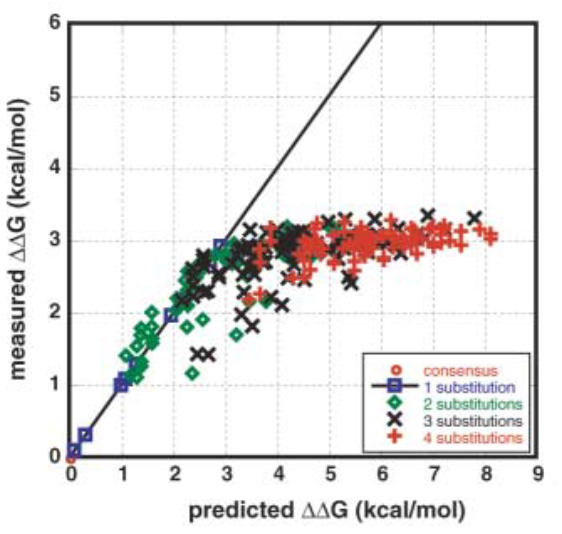
\includegraphics{graphics/predict_failure}}
\caption{\textbf{Energy predictions fail consistently for multiple bp mutants.} Data from Ref. \cite{Maerkl2007} show that predictions made by adding together the energy deviations measured for single bp mutants fail dramatically for multiple bp mutants. }
\label{fig:predict_failure}
\end{center}
\end{figure}

\noindent By contrast, we might think of our models as using ``averaged''
independence. Our single bp mutation data do \textit{not} fall directly
on the line (see Figure \ref{fig:pred_v_fit}). This is because each position of
our energy matrix, rather than being based on a single measurement, is a fitted
value based on many mutant sequences in which the mutation in question is
present with a large selection of other mutations. Any epistatic effects between
this mutation and other mutations will be captured in the mutation's fitted
energy value. Thus, it represents an ``average'' energy taken over many data
points. \\

\noindent Though we do not have data for our 3+ bp mutants yet, I would not be
surprised to find that our data points for these mutants lie loosely along the
line rather than deviating sharply as is seen in Figure \ref{fig:predict_failure}. If this turns out to be the case, I expect it to be
a consequence of using an averaged energy model rather than a strict model. This would be an advantage of our method; because we are able to gather such a large amount of data relatively easily, we can consistently create these averaged models which allow us to make predictions that deviate significantly from the starting sequence. \\

\noindent To support this explanation, I would want to measure the binding energy deviations caused by a collection of single bp mutants and then compare the strict linear predictions produced from these measurements against the averaged linear predictions from the energy matrix. Unfortunately, our collection of mutants was designed to lie between O1 and O2, but it was not necessarily designed with specific single bp mutations in mind. That is, the 2+ bp mutants are not combinations of the mutations chosen for the 1 bp mutants. So, in order to perform these additional experiments we would have to design new operators from scratch, build the constructs, and perform the flow cytometry measurements. \\

\noindent \textbf{Status:} Not started.\\

\noindent \textbf{Timeline:} My experiment calendar is full through the end of October. So, the new constructs could be made in November and the flow experiments could be completed in December.


\bibliographystyle{unsrt}
\bibliography{library}

\end{document}
